\documentclass[tikz,border=10pt]{standalone}
\usetikzlibrary{arrows.meta, positioning, calc, decorations.pathreplacing}
\usepackage{amsmath}
\usepackage{amssymb}

\begin{document}
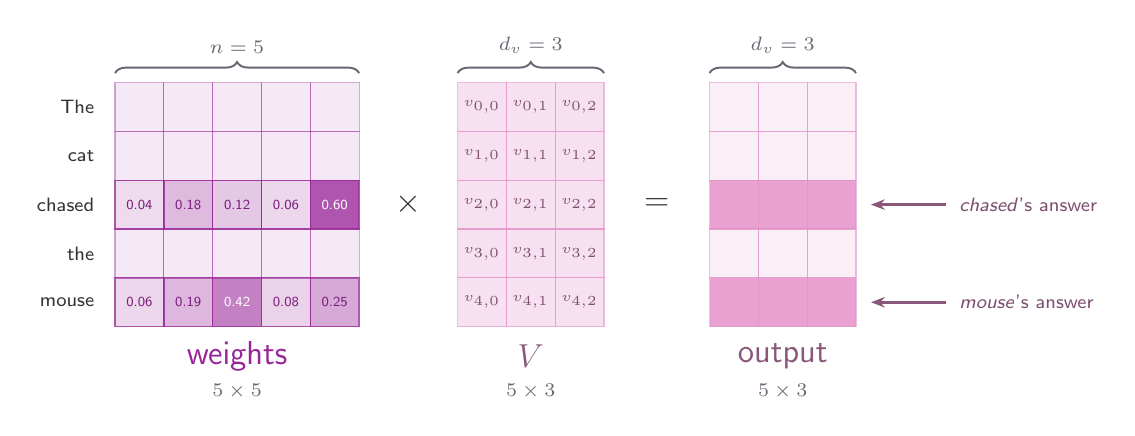
\begin{tikzpicture}[
    every node/.style={font=\sffamily},
]

\definecolor{c1}{HTML}{15173D}
\definecolor{c2}{HTML}{982598}   % the weights
\definecolor{c3}{HTML}{E491C9}   % the values, and the answer
\definecolor{c4}{HTML}{F1E9E9}
\definecolor{axiscolor}{HTML}{333333}
\definecolor{labelcolor}{HTML}{6B6472}

\def\cs{0.62}

% ================================================================
%   weights  top-left (0, 4.2)      5 x 5
%   V        top-left (4.35, 4.2)   5 x 3
%   output   top-left (7.55, 4.2)   5 x 3
%   the shaded row is "chased", whose weights are 0.04 .. 0.60
% ================================================================

% ---------------------------------------------------------------- weights
\foreach \r in {0,...,4} {
    \foreach \c in {0,...,4} {
        \pgfmathsetmacro{\op}{ifthenelse(\r==2 || \r==4, 0.0, 0.10)}
        \fill[c2, opacity=\op] (\c*\cs, 4.2-\r*\cs-\cs) rectangle ++(\cs, \cs);
        \draw[c2, opacity=0.4, line width=0.4pt]
            (\c*\cs, 4.2-\r*\cs-\cs) rectangle ++(\cs, \cs);
    }
}
% two rows are followed through: chased (row 2) and mouse (row 4)
\foreach \v [count=\c from 0] in {0.04, 0.18, 0.12, 0.06, 0.60} {
    \pgfmathsetmacro{\op}{0.12 + 1.1*\v}
    \fill[c2, opacity=\op] (\c*\cs, 4.2-2*\cs-\cs) rectangle ++(\cs, \cs);
    \draw[c2, opacity=0.6, line width=0.5pt]
        (\c*\cs, 4.2-2*\cs-\cs) rectangle ++(\cs, \cs);
    % dark fills need light numerals
    \pgfmathsetmacro{\vv}{\v}
    \ifdim\vv pt>0.39pt \colorlet{celltext}{white}
    \else \colorlet{celltext}{c2!80!black}\fi
    \node[font=\sffamily\tiny, text=celltext]
        at (\c*\cs+0.5*\cs, 4.2-2*\cs-0.5*\cs) {\v};
}
\foreach \v [count=\c from 0] in {0.06, 0.19, 0.42, 0.08, 0.25} {
    \pgfmathsetmacro{\op}{0.12 + 1.1*\v}
    \fill[c2, opacity=\op] (\c*\cs, 4.2-4*\cs-\cs) rectangle ++(\cs, \cs);
    \draw[c2, opacity=0.6, line width=0.5pt]
        (\c*\cs, 4.2-4*\cs-\cs) rectangle ++(\cs, \cs);
    \pgfmathsetmacro{\vv}{\v}
    \ifdim\vv pt>0.39pt \colorlet{celltext}{white}
    \else \colorlet{celltext}{c2!80!black}\fi
    \node[font=\sffamily\tiny, text=celltext]
        at (\c*\cs+0.5*\cs, 4.2-4*\cs-0.5*\cs) {\v};
}
\node[font=\sffamily\large, text=c2] at (1.55, 0.72) {weights};
\node[font=\sffamily\scriptsize, text=labelcolor] at (1.55, 0.28) {$5 \times 5$};

\draw[decorate, decoration={brace, amplitude=4pt}, labelcolor, line width=0.7pt]
    (0, 4.32) -- (3.1, 4.32);
\node[font=\sffamily\scriptsize, text=labelcolor, anchor=south] at (1.55, 4.45)
    {$n = 5$};

\foreach \w/\r in {The/0, cat/1, chased/2, the/3, mouse/4} {
    \node[font=\sffamily\scriptsize, text=axiscolor, anchor=east]
        at (-0.14, 4.2-\r*\cs-0.5*\cs) {\w};
}

\node[font=\sffamily\large, text=axiscolor] at (3.72, 2.65) {$\times$};

% ---------------------------------------------------------------- V
\foreach \r in {0,...,4} {
    \foreach \c in {0,1,2} {
        % uniform: both example rows draw on the whole of V, so shading it for
        % one of them would be misleading
        \fill[c3, opacity=0.28] (4.35+\c*\cs, 4.2-\r*\cs-\cs) rectangle ++(\cs, \cs);
        \draw[c3, opacity=0.6, line width=0.4pt]
            (4.35+\c*\cs, 4.2-\r*\cs-\cs) rectangle ++(\cs, \cs);
        \node[font=\sffamily\tiny, text=c3!55!black]
            at (4.35+\c*\cs+0.5*\cs, 4.2-\r*\cs-0.5*\cs) {$v_{\r,\c}$};
    }
}
\node[font=\sffamily\large, text=c3!60!black] at (5.28, 0.72) {$V$};
\node[font=\sffamily\scriptsize, text=labelcolor] at (5.28, 0.28) {$5 \times 3$};

\draw[decorate, decoration={brace, amplitude=4pt}, labelcolor, line width=0.7pt]
    (4.35, 4.32) -- (6.21, 4.32);
\node[font=\sffamily\scriptsize, text=labelcolor, anchor=south] at (5.28, 4.45)
    {$d_v = 3$};

\node[font=\sffamily\large, text=axiscolor] at (6.88, 2.65) {$=$};

% ---------------------------------------------------------------- output
\foreach \r in {0,...,4} {
    \foreach \c in {0,1,2} {
        \pgfmathsetmacro{\op}{ifthenelse(\r==2 || \r==4, 0.85, 0.14)}
        \fill[c3, opacity=\op] (7.55+\c*\cs, 4.2-\r*\cs-\cs) rectangle ++(\cs, \cs);
        \draw[c3, opacity=0.6, line width=0.4pt]
            (7.55+\c*\cs, 4.2-\r*\cs-\cs) rectangle ++(\cs, \cs);
    }
}
\node[font=\sffamily\large, text=c3!60!black] at (8.48, 0.72) {output};
\node[font=\sffamily\scriptsize, text=labelcolor] at (8.48, 0.28) {$5 \times 3$};

\draw[decorate, decoration={brace, amplitude=4pt}, labelcolor, line width=0.7pt]
    (7.55, 4.32) -- (9.41, 4.32);
\node[font=\sffamily\scriptsize, text=labelcolor, anchor=south] at (8.48, 4.45)
    {$d_v = 3$};

\draw[-{Stealth[length=5pt]}, line width=1.0pt, c3!60!black]
    (10.55, 2.65) -- (9.6, 2.65);
\node[font=\sffamily\scriptsize, text=c3!55!black, anchor=west, align=left]
    at (10.6, 2.65) {\emph{chased}'s answer};

\draw[-{Stealth[length=5pt]}, line width=1.0pt, c3!60!black]
    (10.55, 1.41) -- (9.6, 1.41);
\node[font=\sffamily\scriptsize, text=c3!55!black, anchor=west, align=left]
    at (10.6, 1.41) {\emph{mouse}'s answer};

\end{tikzpicture}
\end{document}
